\section{Binary Planar Partitions}
\subsection{Forklaring af algoritmen}

Givet en mængde af ikke-overlappende input-segmenter $S$ og initielt $R = \R^2$, så fungerer algoritmen således:\\


\texttt{AutoPartition}$(S, R)$
\begin{itemize}
    \item Hvis $|S| \leq 1$, så returner blad $(S, R)$.
    \item Vælg segment $s \in S$ og lad $l(s)$ være en linje gennem $s$.
    \item Split $R$ langs $l(s)$ i $R_1$ og $R_2$.
    \item For $i=1,2$, så lad $S_i = \{ s' \in R_i | s' \in S \land s' \nsubseteq l(s)  \}$ (dvs. sættet af $s'$ der er i $R_i$ hvor de også var i input $S$ og ikke skærer eller ligger ovenpå $l(s)$).
    \item For $i=1,2$, så lad $T_i = $ \texttt{AutoPartition}$(S_i, R_i)$
    \item Returner træet\\
    \begin{forest}
        [$(l(s)\text{, } R)$
          [$T_1$]
          [$T_2$]
        ]
    \end{forest}
\end{itemize}

\texttt{RandAutoPartition}$(S)$
\begin{itemize}
    \item Vælg uniformt en tilfældig permutation $\pi$ af $\{1, 2, ..., n \}$ fra de $n!$ mulige permutationer.
    \item Kør rekursiv algoritme, men vælg segmenter i forhold til permutation $\pi$.
\end{itemize}

Et eksempel følger her med uddybende forklaringer nedenfor:
\begin{figure}[H]
	\centering
	\begin{subfigure}[b]{0.48\textwidth}
		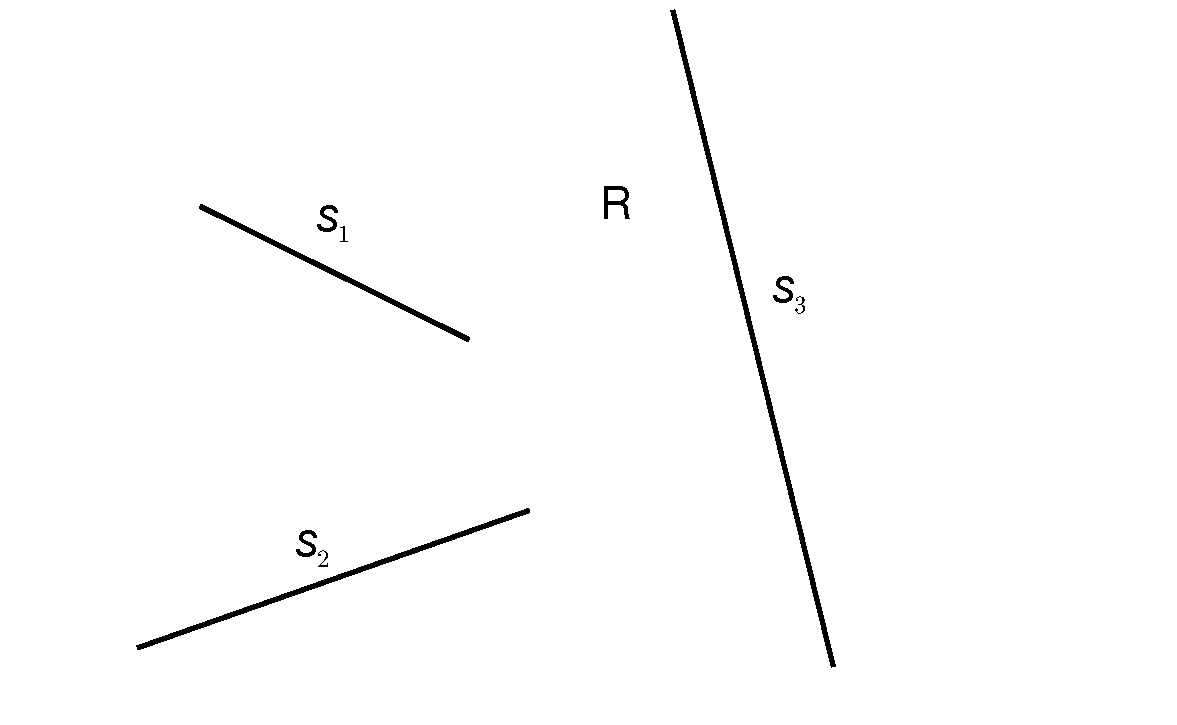
\includegraphics[width=\textwidth]{bpp-1.pdf}
		\caption{Algoritmen kaldes på $R = \R^2$ og $S = \{s_2, s_1, s_3 \}$.}
		\label{fig:bpp-1}
	\end{subfigure}
	~
	\begin{subfigure}[b]{0.48\textwidth}
		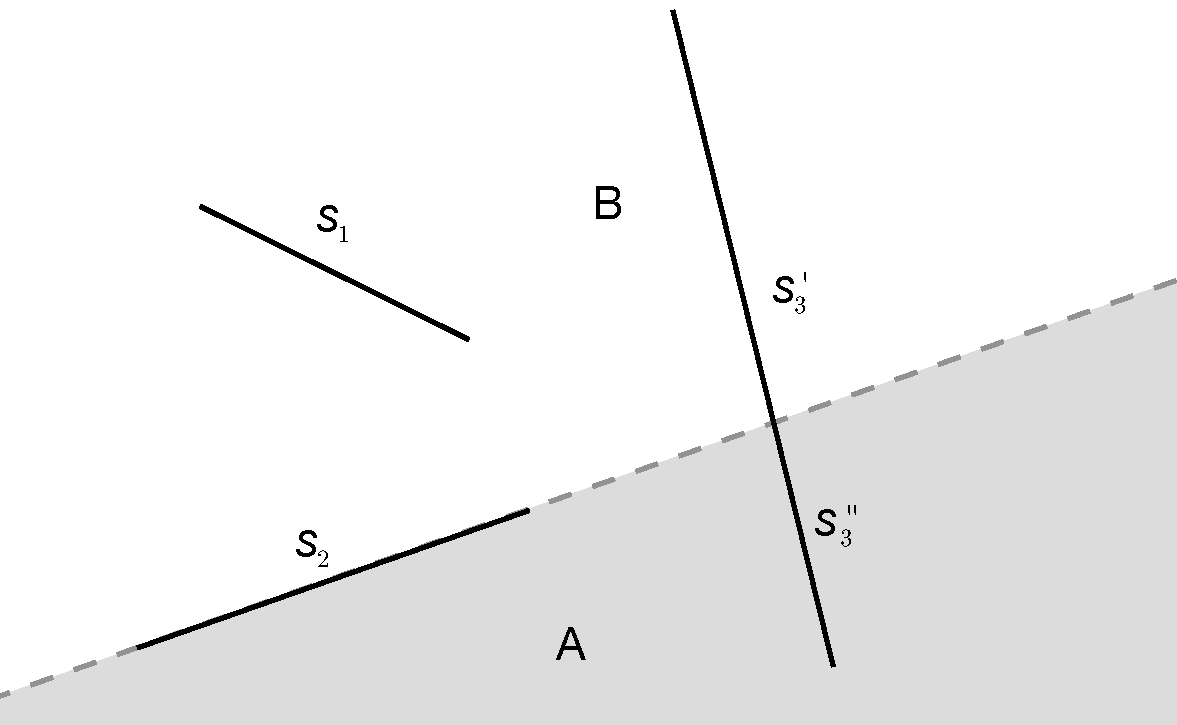
\includegraphics[width=\textwidth]{bpp-2.pdf}
        \caption{Vi vælger segmentet $s_2$.}
		\label{fig:bpp-2}
	\end{subfigure}
	~
	\begin{subfigure}[b]{0.48\textwidth}
		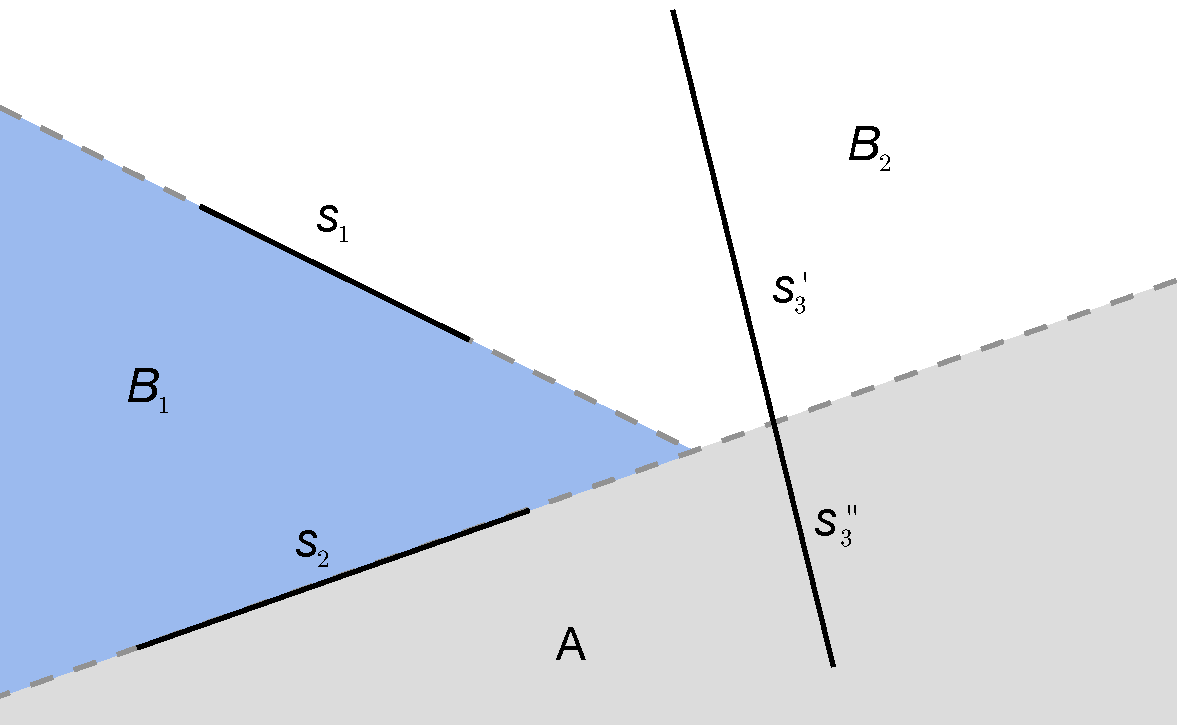
\includegraphics[width=\textwidth]{bpp-3.pdf}
		\caption{Vi vælger segmentet $s_1$.}
		\label{fig:bpp-3}
	\end{subfigure}
	~
	\begin{subfigure}[b]{0.48\textwidth}
		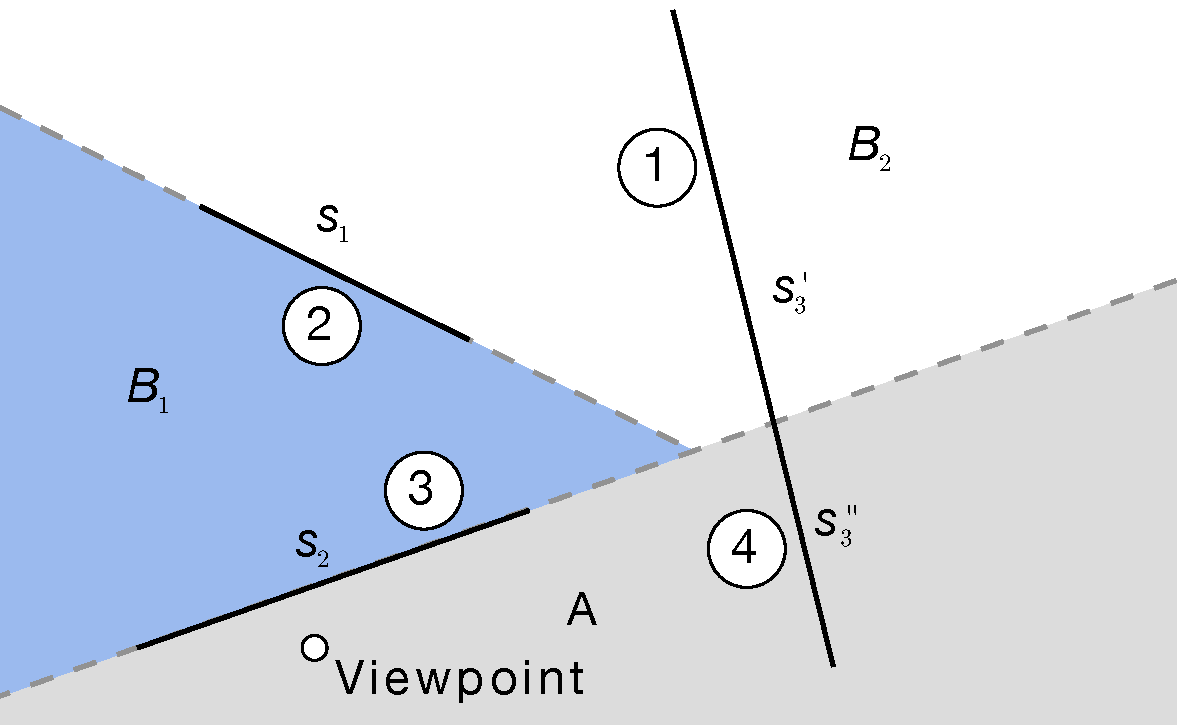
\includegraphics[width=\textwidth]{bpp-4.pdf}
		\caption{Rækkefølgen linjesegmenterne skal tegnes i.}
		\label{fig:bpp-4}
	\end{subfigure}
	\caption{Eksempel på kørsel af \texttt{RandAutoPartition}}
	\label{fig:bpp}
\end{figure}

\begin{itemize}
    \item[\textbf{(a)}] Initielt kald. Vores træ er tomt og $R$ er markeret med hvid.

    \item[\textbf{(b)}] Vi vælger $s_2$ og ser, at $l(s_2)$ rammer ind i $s_3$, så den splittes i to nye dellinjesegmenter, $s_3'$ og $s_3''$. Derudover splitter vi $R$ til $A = \{s_3'' \}$ og $B = \{s_1, s_3' \}$, hvor $A$ er markeret med grå på figuren og $B$ er markeret med hvid. For de rekursive kald den laver i niveauet lige under sig vil vi få følgende træ (bemærk dog, at i praksis vil hele venstre side blive beregnet først):\\
    \begin{forest}
        [$(l(s_2)\text{, } \R^2)$
          [$(l(s_1)\text{, } B)$]
          [$(\{ s_3''\}\text{, } A)$]
        ]
    \end{forest}

    \item[\textbf{(c)}] Vi vælger $s_1$. Når vi rammer et tidligere linje, her $l(s_2)$, skal vi ikke forlænge linjen yderligere. Derfor splitter den ikke nogle linjesegmenter. Den deler stadig arealet $B$ op i $B_1 = \emptyset$ (markeret med lyseblåt) og $B_2 = \{s_3' \}$ (markeret med hvid). Vi får træet:\\
    \begin{forest}
        [$(l(s_2)\text{, } \R^2)$
          [$(l(s_1)\text{, } B)$
            [$(\emptyset \text{, } B_1)$]
            [$(\{ s_3'\}\text{, } B_2)$]
          ]
          [$(\{ s_3''\}\text{, } A)$]
        ]
    \end{forest}

    \item[\textbf{(d)}] Træet blev beregnet færdigt i (c). Her er så markeret i hvilken rækkefølge de forskellige linjesegmenter $\{s_1, s_2, s_3', s_3''\}$ skal tegnes i idet vi står ved viewpoint'et markeret på figuren.
\end{itemize}

\subsection{Forventet antal linjesegmenter i output-træ}
Lad $S$ være mængden af input-segmenter og lad $n = |S|$.


Vi indfører nu en indikatorvariabel $X_{s, s'}$ for alle $s, s' \in S$ hvor $s \neq s'$ og:
\begin{align*}
    X_{s, s'} =
    \begin{cases}
        1, & \text{hvis $s$ eller delsegment af $s$ splitter $s'$ eller delsegment af $s'$}\\
        0  & \text{ellers}
    \end{cases}
\end{align*}

Bemærk at rækkefølgen på $s$ og $s'$ ikke er ligegyldig. F.eks. ville vi for \ref{fig:bpp} have, at $X_{s_2, s_3} = 1$ mens $X_{s_3, s_2} = 0$.

Hvis vi nu med den stokastiske variabel $X$ beskriver antal delsegmenter i outputtet (f.eks. $X = 4$ for \ref{fig:bpp}), så må det svare til antal linjesegmenter $n$ der er til at starte med plus summen af alle indikatorvariablerne, da de netop har værdien 1 når de splitter et delsegment (hvilket resulterer i endnu et delsegment) og 0 ellers, hvorved vi får følgende idet vi bruger linearity of expectation:

\begin{align}
    X     &= n + \sum_{s \in S} \sum_{s' \in S \backslash \{ s\}} X_{s, s'} \nonumber \\
    \e[X] &= n + \sum_{s \in S} \sum_{s' \in S \backslash \{ s\}} \e[X_{s, s'}]
           = n + \sum_{s \in S} \sum_{s' \in S \backslash \{ s\}} \P[X_{s, s'} = 1] \label{eq:bpp-X-init}
\end{align}

Lad os nu betragte et fast $s$ og $s'$ og antage, at $l(s)$ skærer $s'$.
\begin{figure}[H]
    \begin{center}
    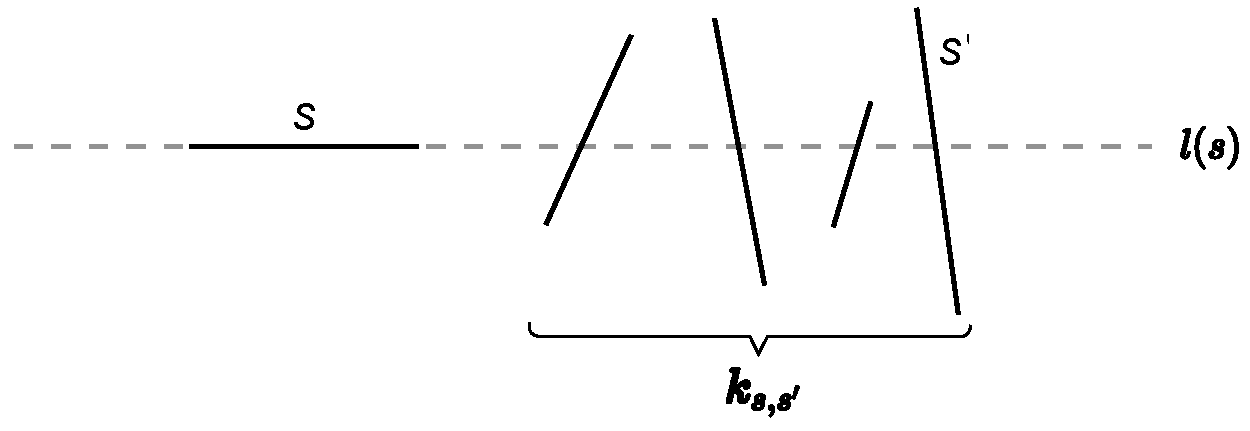
\includegraphics[width=0.6\textwidth]{bpp-split.pdf}
    \end{center}
    \caption{Et $s$, hvor $l(s)$ skærer $s'$ og $k_{s, s'} = 4$}
    \label{fig:bpp-split}
\end{figure}


Med $k_{s, s'}$ definerer vi antallet af linjesegmenter der lægger imellem $s$ og $s'$, eksklusiv $s$ og inklusiv $s'$. Vi kan regne ud, at $1 \leq k_{s, s'} \leq n-1$, da den altid som minimum vil inkludere $s'$ og potentielt kan inkludere alle linjesegmenter i $S$ pånær $s$.\\

Hvis vi nu har, at $s$ splitter $s'$, så må det nødvendigvis betyde, at $s$ er først i permutationen blandt de $k_{s, s'} + 1$ segmenter i tegningen. Heraf følger, at:
\begin{align} \label{eq:bpp-prob-split}
    \P[X_{s, s'} = 1] = \P[\text{$s$ splitter $s'$}] \leq \frac{1}{k_{s, s'} + 1}
\end{align}
\textbf{TODO: Hvorfor '$\leq$'-tegnet og ikke bare '='?}


Nu kan vi benytte \cref{eq:bpp-prob-split} til at regne videre på \cref{eq:bpp-X-init}:
\begin{align}
\e[X] &\leq n + \sum_{s \in S} \sum_{s' \in S \backslash \{ s\}} \frac{1}{k_{s, s'}+1} \nonumber \\
      &\leq n + \sum_{s \in S} \sum_{k=1}^{n-1} 2 * \frac{1}{k+1} \label{eq:bpp-X-weird} \\
      &= n + 2 * \sum_{s \in S} \sum_{k=2}^{n} \frac{1}{k} \label{eq:bpp-mindre} \\
      &\leq n + 2 * \sum_{s \in S} \sum_{k=1}^{n} \frac{1}{k} \nonumber \\
      &= n + 2n \sum_{k=1}^{n} \frac{1}{k} \label{eq:bpp-sum-til-n} \\
      &= n + 2n H_n \label{eq:bpp-harmonic} \\
      &= O(n \lg n) \label{eq:bpp-final}
\end{align}

%I \cref{eq:bpp-X-weird} benytter vi, at for $k = 1,2, ..., n-1$ kan der højest være to segmenter $s'$, så $k_{s, s'} = k$. \textbf{TODO: Hvad?... Uddyb}.


Husk at $k_{s, s'}$ betegner antallet af linje segmenter $s$ går igennem indtil den når $s’$ (med $s’$). Så lad $k=1,2,..n-1$, også har vi at $k_{s,s’} = k$. Vi kan have linje segmenter på venstre og højre siden af s, som kan ses i \cref{fig:bpp-split-k}. Dvs. at der højst kan være 2 segmenter $s'$ - altså 2 forskellige muligheder for denne og vi er altså nødt til at tælle denne sandsynlighed dobbelt. Dette er hvad vi ser i \cref{eq:bpp-X-weird}.


\begin{figure}[H]
    \begin{center}
    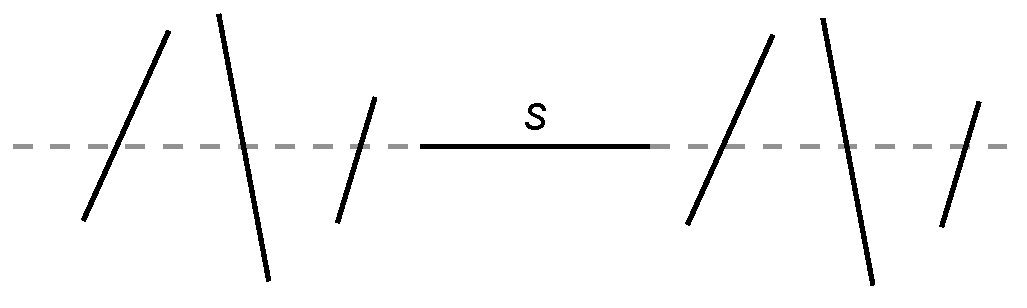
\includegraphics[width=0.5\textwidth]{bpp-split-k.pdf}
    \end{center}
    \caption{Vi ser, at der højest kan være to segmenter $s'$ for $s$}
    \label{fig:bpp-split-k}
\end{figure}

I \cref{eq:bpp-mindre} ganger vi 2 udenfor sumtegnene. Derudover lader vi andet sumtegn iterere over værdier der er en højere for at få en pænere brøk.\\
I \cref{eq:bpp-sum-til-n} - \cref{eq:bpp-final} benytter vi det $n$'te harmoniske tal $H_n = \ln n + \Theta(1)$.\\

Hermed har vi altså vist, at den forventede størrelse $\e[X]$ af vores output-træ vil være $O(n \lg n)$.
